\chapter{Research Findings}
For the purpose of bencharking the performance of the algorithms, a total of five stocks from the basket of uncorrelated stocks were selected. These were MSFT, CDE, NAVB, HRG, and HL. 

\begin{center}
    \includegraphics[width=\textwidth]{stocks.png}
    \captionof{figure}{Basket of stocks}
    \label{fig:nonfloat}
\end{center}

\begin{center}
    \begin{tabular}{ | l | l | l | | l | l | l | p{5cm} |}
    \hline
     & MSFT & CDE & NAVB & HRG & HL \\ \hline
    Mean & 16.983 & 57.716 & 3.000 & 13.328 & 7.154 \\ \hline
    Median & 18.656 & 36.700 & 1.250 & 7.190 & 6.196 \\ \hline
    Maximum & 63.620 & 213.178 & 22.000 & 89.340 & 23.830 \\ \hline
    Minimum & 0.061 & 1.730 & 0.080 & 1.725 & 0.486 \\ \hline
    Variance & 204.707 & 2807.852 & 18.445 & 249.105 & 18.445 \\ \hline
    Standard Deviation & 14.308 & 52.989 & 4.29 & 15.783 & 4.295 \\ \hline
    Skewness & 0.716 & 0.918 & 2.213 & 2.708 & 0.651 \\ \hline
    Kurtosis & 0.250 & -0.550 & 4.193 & 6.865 & -0.081 \\ \hline
    \hline
    \end{tabular}
    \captionof{table}{Equities Descriptive Statistics}
    \label{table:nonfloat}
\end{center}

\section{Time Series Analysis}

\subsection{Random Walk}

\begin{center}
    \includegraphics[width=\textwidth]{MSFT-time-series.png}
    \captionof{figure}{MSFT time series analysis}
    \label{fig:nonfloat}
\end{center}

\begin{center}
    \includegraphics[width=\textwidth]{MSFT-histogram.png}
    \captionof{figure}{MSFT histogram of returns}
    \label{fig:nonfloat}
\end{center}

\begin{center}  
    \includegraphics[width=\textwidth]{CDE-time-series.png}
    \captionof{figure}{CDE time series analysis}
    \label{fig:nonfloat}
\end{center}

\begin{center}  
    \includegraphics[width=\textwidth]{CDE-histogram.png}
    \captionof{figure}{CDE histogram of returns}
    \label{fig:nonfloat}
\end{center}

\begin{center}
  
    \includegraphics[width=\textwidth]{NAVB-time-series.png}
    \captionof{figure}{NAVB time series analysis}
    \label{fig:nonfloat}
\end{center}

\begin{center}
  
    \includegraphics[width=\textwidth]{NAVB-histogram.png}
    \captionof{figure}{NAVB histogram of returns}
    \label{fig:nonfloat}
\end{center}

\begin{center}
    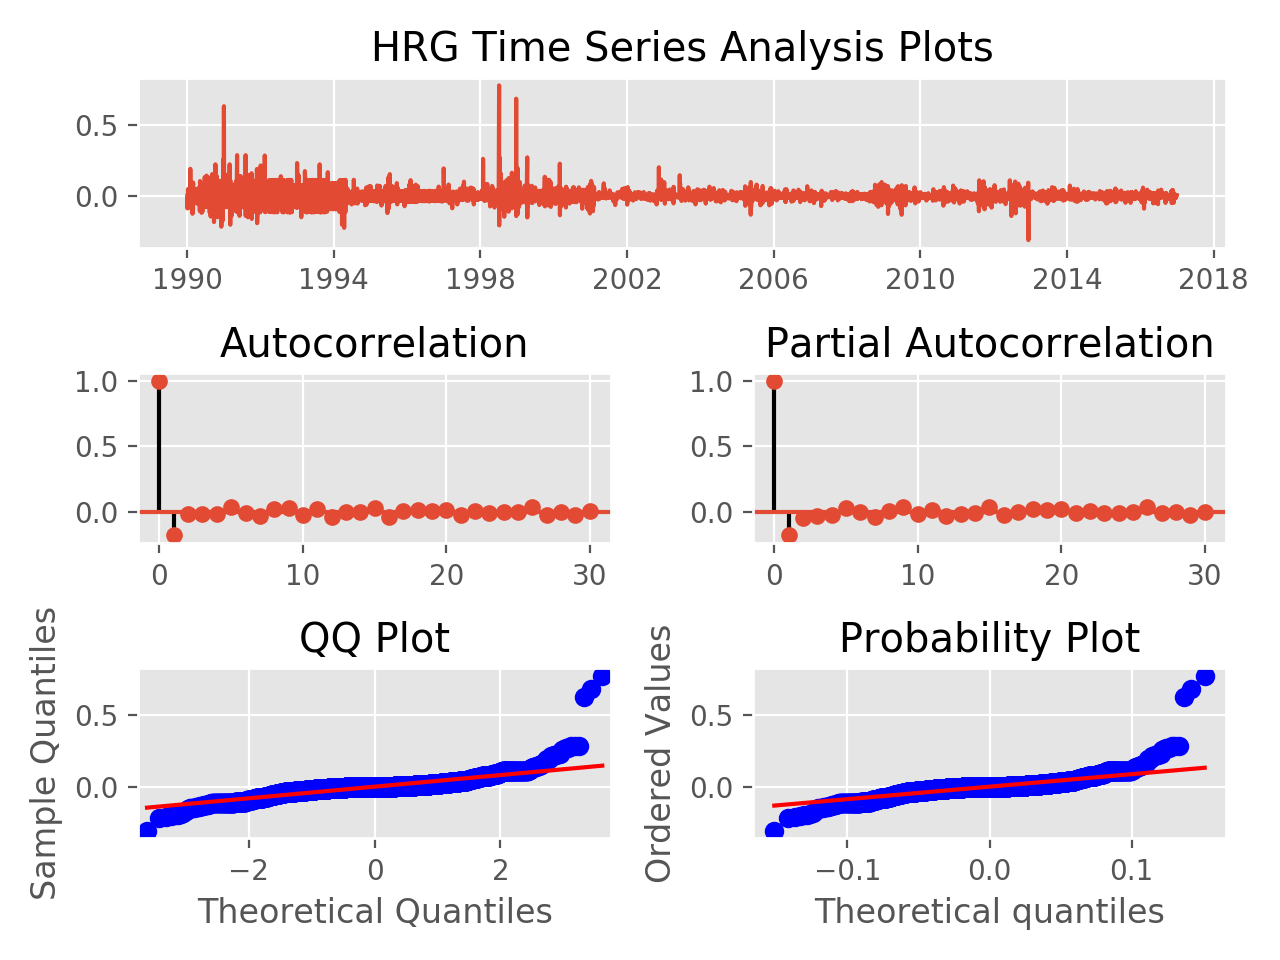
\includegraphics[width=\textwidth]{HRG-time-series.png}
    \captionof{figure}{HRG time series analysis}
    \label{fig:nonfloat}
\end{center}

\begin{center}  
    \includegraphics[width=\textwidth]{HRG-histogram.png}
    \captionof{figure}{HRG histogram of returns}
    \label{fig:nonfloat}
\end{center}

\begin{center}
    \includegraphics[width=\textwidth]{HL-time-series.png}
    \captionof{figure}{HL time series analysis}
    \label{fig:nonfloat}
\end{center}

\begin{center}  
    \includegraphics[width=\textwidth]{HL-histogram.png}
    \captionof{figure}{HL histogram of returns}
    \label{fig:nonfloat}
\end{center}

\subsection{Ordinary Least Squares (OLS)}
MSFT scored a mean absolute error regression loss of 0.810, and a coefficient of determination of 0.991.

\begin{center}
    \includegraphics[width=\textwidth]{MSFT-OLS-In-Sample-Prediction.png}
    \captionof{figure}{MSFT OLS in-sample prediction}
    \label{fig:nonfloat}
\end{center}

\begin{center}  
    \includegraphics[width=\textwidth]{100-Day-MSFT-OLS-Out-of-Sample-Forecast.png}
    \captionof{figure}{100 day MSFT OLS in-sample forecast}
    \label{fig:nonfloat}
\end{center}

CDE scored a mean absolute error regression loss of 0.985, and a coefficient of determination of 0.973.

\begin{center}
    \includegraphics[width=\textwidth]{CDE-OLS-In-Sample-Prediction.png}
    \captionof{figure}{CDE OLS in-sample prediction}
    \label{fig:nonfloat}
\end{center}

\begin{center}
    \includegraphics[width=\textwidth]{100-Day-CDE-OLS-Out-of-Sample-Forecast.png}
    \captionof{figure}{100 Day CDE OLS out of sample forecast}
    \label{fig:nonfloat}
\end{center}

NAVB scored a mean absolute error regression loss of 0.124, and a coefficient of determination of 0.966.

\begin{center}  
    \includegraphics[width=\textwidth]{NAVB-OLS-In-Sample-Prediction.png}
    \captionof{figure}{NAVB OLS in-sample prediction}
    \label{fig:nonfloat}
\end{center}

\begin{center}
  
    \includegraphics[width=\textwidth]{100-Day-NAVB-OLS-Out-of-Sample-Forecast.png}
    \captionof{figure}{100 day NAVB OLS in-sample forecast}
    \label{fig:nonfloat}
\end{center}

HRG scored a mean absolute error regression loss of 0.291, and a coefficient of determination of 0.986.

\begin{center}  
    \includegraphics[width=\textwidth]{HRG-OLS-In-Sample-Prediction.png}
    \captionof{figure}{HRG OLS in-sample prediction}
    \label{fig:nonfloat}
\end{center}

\begin{center}
    \includegraphics[width=\textwidth]{100-Day-HRG-OLS-Out-of-Sample-Forecast.png}
    \captionof{figure}{100 day HRG OLS in-sample forecast}
    \label{fig:nonfloat}
\end{center}

HL scored a mean absolute error regression loss of 0.336, and a coefficient of determination of 0.963.

\begin{center}  
    \includegraphics[width=\textwidth]{HL-OLS-In-Sample-Prediction.png}
    \captionof{figure}{HL OLS in-sample prediction}
    \label{fig:nonfloat}
\end{center}

\begin{center}
    \includegraphics[width=\textwidth]{100-Day-HL-OLS-Out-of-Sample-Forecast.png}
    \captionof{figure}{100 day HL OLS in-sample forecast}
    \label{fig:nonfloat}
\end{center}

\subsection{Auto Regressive (AR)}

MSFT scored sharpe ratios of 1.152 for the original returns, and -34.641 for the predicted returns in the in-sample test.

\begin{center}  
    \includegraphics[width=\textwidth]{MSFT-AR-time-series.png}
    \captionof{figure}{MSFT AR time series analysis}
    \label{fig:nonfloat}
\end{center}

\begin{center}
    \includegraphics[width=\textwidth]{MSFT-AR-histogram.png}
    \captionof{figure}{MSFT AR histogram of returns}
    \label{fig:nonfloat}
\end{center}

\begin{center}  
    \includegraphics[width=\textwidth]{MSFT-AR-In-Sample-Return-Prediction.png}
    \captionof{figure}{MSFT AR in-sample returns prediction}
    \label{fig:nonfloat}
\end{center}

\begin{center}
    \includegraphics[width=\textwidth]{100-Day-MSFT-AR-Out-of-Sample-Return-Forecast.png}
    \captionof{figure}{100 day MSFT AR in-sample returns forecast}
    \label{fig:nonfloat}
\end{center}

CDE scored sharpe ratios of -1.050 for the original returns, and -0.239 for the predicted returns in the in-sample test.

\begin{center}
    \includegraphics[width=\textwidth]{CDE-AR-time-series.png}
    \captionof{figure}{CDE AR time series analysis}
    \label{fig:nonfloat}
\end{center}

\begin{center}
    \includegraphics[width=\textwidth]{CDE-AR-histogram.png}
    \captionof{figure}{CDE AR histogram of returns}
    \label{fig:nonfloat}
\end{center}

\begin{center}
    \includegraphics[width=\textwidth]{CDE-AR-In-Sample-Return-Prediction.png}
    \captionof{figure}{CDE AR in-sample returns prediction}
    \label{fig:nonfloat}
\end{center}

\begin{center}
    \includegraphics[width=\textwidth]{100-Day-CDE-AR-Out-of-Sample-Return-Forecast.png}
    \captionof{figure}{100 day CDE AR in-sample returns forecast}
    \label{fig:nonfloat}
\end{center}

NAVB scored sharpe ratios of -0.410 for the original returns, and 0.124 for the predicted returns in the in-sample test.

\begin{center}
    \includegraphics[width=\textwidth]{NAVB-AR-time-series.png}
    \captionof{figure}{NAVB AR time series analysis}
    \label{fig:nonfloat}
\end{center}

\begin{center}
    \includegraphics[width=\textwidth]{NAVB-AR-histogram.png}
    \captionof{figure}{NAVB AR histogram of returns}
    \label{fig:nonfloat}
\end{center}

\begin{center}
    \includegraphics[width=\textwidth]{NAVB-AR-In-Sample-Return-Prediction.png}
    \captionof{figure}{NAVB AR in-sample returns prediction}
    \label{fig:nonfloat}
\end{center}

\begin{center}
    \includegraphics[width=\textwidth]{100-Day-NAVB-AR-Out-of-Sample-Return-Forecast.png}
    \captionof{figure}{100 day NAVB AR in-sample returns forecast}
    \label{fig:nonfloat}
\end{center}

HRG scored sharpe ratios of 0.627 for the original returns, and -2.603 for the predicted returns in the in-sample test.

\begin{center}  
    \includegraphics[width=\textwidth]{HRG-AR-time-series.png}
    \captionof{figure}{HRG AR time series analysis}
    \label{fig:nonfloat}
\end{center}

\begin{center}
  
    \includegraphics[width=\textwidth]{HRG-AR-histogram.png}
    \captionof{figure}{HRG AR histogram of returns}
    \label{fig:nonfloat}
\end{center}

\begin{center}
    \includegraphics[width=\textwidth]{HRG-AR-In-Sample-Return-Prediction.png}
    \captionof{figure}{HL AR in-sample returns prediction}
    \label{fig:nonfloat}
\end{center}

\begin{center}
    \includegraphics[width=\textwidth]{100-Day-HRG-AR-Out-of-Sample-Return-Forecast.png}
    \captionof{figure}{100 day HRG AR in-sample returns forecast}
    \label{fig:nonfloat}
\end{center}

HL scored sharpe ratios of 0.695 for the original returns, and -1.880 for the predicted returns in the in-sample test.

\begin{center}  
    \includegraphics[width=\textwidth]{HL-AR-time-series.png}
    \captionof{figure}{HL AR time series analysis}
    \label{fig:nonfloat}
\end{center}

\begin{center}
    \includegraphics[width=\textwidth]{HL-AR-histogram.png}
    \captionof{figure}{HL AR histogram of returns}
    \label{fig:nonfloat}
\end{center}

\begin{center}
  
    \includegraphics[width=\textwidth]{HL-AR-In-Sample-Return-Prediction.png}
    \captionof{figure}{HL AR in-sample returns prediction}
    \label{fig:nonfloat}
\end{center}

\begin{center}
  
    \includegraphics[width=\textwidth]{100-Day-HL-AR-Out-of-Sample-Return-Forecast.png}
    \captionof{figure}{100 day HL AR in-sample returns forecast}
    \label{fig:nonfloat}
\end{center}

\subsection{Moving Average (MA)}

MSFT scored sharpe ratios of 0.358 for the original returns, and -5.610 for the predicted returns in the in-sample test.

\begin{center}
    \includegraphics[width=\textwidth]{MSFT-MA-time-series.png}
  \captionof{figure}{MSFT MA time series analysis}
  \label{fig:nonfloat}
\end{center}

\begin{center}
    \includegraphics[width=\textwidth]{MSFT-MA-histogram.png}
    \captionof{figure}{MSFT MA histogram of returns}
    \label{fig:nonfloat}
\end{center}

\begin{center}  
    \includegraphics[width=\textwidth]{MSFT-MA-In-Sample-Return-Prediction.png}
    \captionof{figure}{MSFT MA in-sample returns prediction}
    \label{fig:nonfloat}
\end{center}

\begin{center}  
    \includegraphics[width=\textwidth]{100-Day-MSFT-MA-Out-of-Sample-Return-Forecast.png}
    \captionof{figure}{100 day MSFT MA in-sample returns forecast}
    \label{fig:nonfloat}
\end{center}

CDE scored sharpe ratios of -0.199 for the original returns, and -0.760 for the predicted returns in the in-sample test.

\begin{center}
    \includegraphics[width=\textwidth]{CDE-MA-time-series.png}
    \captionof{figure}{CDE MA time series analysis}
    \label{fig:nonfloat}
\end{center}

\begin{center}  
    \includegraphics[width=\textwidth]{CDE-MA-histogram.png}
    \captionof{figure}{CDE MA histogram of returns}
    \label{fig:nonfloat}
\end{center}

\begin{center}  
    \includegraphics[width=\textwidth]{CDE-MA-In-Sample-Return-Prediction.png}
    \captionof{figure}{CDE MA in-sample returns prediction}
    \label{fig:nonfloat}
\end{center}

\begin{center}
    \includegraphics[width=\textwidth]{100-Day-CDE-MA-Out-of-Sample-Return-Forecast.png}
    \captionof{figure}{100 day CDE MA in-sample returns forecast}
    \label{fig:nonfloat}
\end{center}

NAVB scored sharpe ratios of -0.067 for the original returns, and 0.590 for the predicted returns in the in-sample test.

\begin{center}  
    \includegraphics[width=\textwidth]{NAVB-MA-time-series.png}
    \captionof{figure}{NAVB MA time series analysis}
    \label{fig:nonfloat}
\end{center}

\begin{center}  
    \includegraphics[width=\textwidth]{NAVB-MA-histogram.png}
    \captionof{figure}{NAVB MA histogram of returns}
    \label{fig:nonfloat}
\end{center}

\begin{center}
    \includegraphics[width=\textwidth]{NAVB-MA-In-Sample-Return-Prediction.png}
    \captionof{figure}{NAVB MA in-sample returns prediction}
    \label{fig:nonfloat}
\end{center}

\begin{center}
    \includegraphics[width=\textwidth]{100-Day-NAVB-MA-Out-of-Sample-Return-Forecast.png}
    \captionof{figure}{100 day NAVB MA in-sample returns forecast}
    \label{fig:nonfloat}
\end{center}

HRG scored sharpe ratios of 0.084 for the original returns, and -1.020 for the predicted returns in the in-sample test.

\begin{center}  
    \includegraphics[width=\textwidth]{HRG-MA-time-series.png}
    \captionof{figure}{HRG MA time series analysis}
    \label{fig:nonfloat}
\end{center}

\begin{center}  
    \includegraphics[width=\textwidth]{HRG-MA-histogram.png}
    \captionof{figure}{HRG MA histogram of returns}
    \label{fig:nonfloat}
\end{center}

\begin{center}
    \includegraphics[width=\textwidth]{HRG-MA-In-Sample-Return-Prediction.png}
    \captionof{figure}{HRG MA in-sample returns prediction}
    \label{fig:nonfloat}
\end{center}

\begin{center}
    \includegraphics[width=\textwidth]{100-Day-HRG-MA-Out-of-Sample-Return-Forecast.png}
    \captionof{figure}{100 day HRG MA in-sample returns forecast}
    \label{fig:nonfloat}
\end{center}

HL scored sharpe ratios of -0.128 for the original returns, and -0.977 for the predicted returns in the in-sample test.

\begin{center}
    \includegraphics[width=\textwidth]{HL-MA-time-series.png}
    \captionof{figure}{HL MA time series analysis}
    \label{fig:nonfloat}
\end{center}

\begin{center}
    \includegraphics[width=\textwidth]{HL-MA-histogram.png}
    \captionof{figure}{HL MA histogram of returns}
    \label{fig:nonfloat}
\end{center}

\begin{center}
    \includegraphics[width=\textwidth]{HL-MA-In-Sample-Return-Prediction.png}
    \captionof{figure}{HL MA in-sample returns prediction}
    \label{fig:nonfloat}
\end{center}

\begin{center}
    \includegraphics[width=\textwidth]{100-Day-HL-MA-Out-of-Sample-Return-Forecast.png}
    \captionof{figure}{100 day HL MA in-sample returns forecast}
    \label{fig:nonfloat}
\end{center}

\subsection{Auto Regressive Moving Average (ARMA)}

HL scored sharpe ratios of 0.537 for the original returns, and -6.485 for the predicted returns in the in-sample test.

\begin{center}  
    \includegraphics[width=\textwidth]{MSFT-ARMA-time-series.png}
    \captionof{figure}{MSFT ARMA time series analysis}
    \label{fig:nonfloat}
\end{center}

\begin{center}
    \includegraphics[width=\textwidth]{MSFT-ARMA-histogram.png}
    \captionof{figure}{MSFT ARMA histogram of returns}
    \label{fig:nonfloat}
\end{center}

\begin{center}
    \includegraphics[width=\textwidth]{MSFT-ARMA-In-Sample-Return-Prediction.png}
    \captionof{figure}{MSFT ARMA in-sample returns prediction}
    \label{fig:nonfloat}
\end{center}

\begin{center}
    \includegraphics[width=\textwidth]{100-Day-MSFT-ARMA-Out-of-Sample-Return-Forecast.png}
    \captionof{figure}{100 day MSFT ARMA in-sample returns forecast}
    \label{fig:nonfloat}
\end{center}

MSFT scored sharpe ratios of -0.128 for the original returns, and -0.977 for the predicted returns in the in-sample test.

\begin{center}
    \includegraphics[width=\textwidth]{CDE-ARMA-time-series.png}
    \captionof{figure}{CDE ARMA time series analysis}
    \label{fig:nonfloat}
\end{center}

\begin{center}
    \includegraphics[width=\textwidth]{CDE-ARMA-histogram.png}
    \captionof{figure}{CDE ARMA histogram of returns}
    \label{fig:nonfloat}
\end{center}

\begin{center}
    \includegraphics[width=\textwidth]{CDE-ARMA-In-Sample-Return-Prediction.png}
    \captionof{figure}{CDE ARMA in-sample returns prediction}
    \label{fig:nonfloat}
\end{center}

\begin{center}
    \includegraphics[width=\textwidth]{100-Day-CDE-ARMA-Out-of-Sample-Return-Forecast.png}
    \captionof{figure}{100 day CDE ARMA in-sample returns forecast}
    \label{fig:nonfloat}
\end{center}

CDE scored sharpe ratios of -0.245 for the original returns, and -0.614 for the predicted returns in the in-sample test.

\begin{center}  
    \includegraphics[width=\textwidth]{NAVB-ARMA-time-series.png}
    \captionof{figure}{NAVB ARMA time series analysis}
    \label{fig:nonfloat}
\end{center}

\begin{center}
    \includegraphics[width=\textwidth]{NAVB-ARMA-histogram.png}
    \captionof{figure}{NAVB ARMA histogram of returns}
    \label{fig:nonfloat}
\end{center}

\begin{center}  
    \includegraphics[width=\textwidth]{NAVB-ARMA-In-Sample-Return-Prediction.png}
    \captionof{figure}{NAVB ARMA in-sample returns prediction}
    \label{fig:nonfloat}
\end{center}

\begin{center}  
    \includegraphics[width=\textwidth]{100-Day-NAVB-ARMA-Out-of-Sample-Return-Forecast.png}
    \captionof{figure}{100 day NAVB ARMA in-sample returns forecast}
    \label{fig:nonfloat}
\end{center}

NAVB scored sharpe ratios of -0.032 for the original returns, and -0.641 for the predicted returns in the in-sample test.

\begin{center}
    \includegraphics[width=\textwidth]{HRG-ARMA-time-series.png}
    \captionof{figure}{HRG ARMA time series analysis}
    \label{fig:nonfloat}
\end{center}

\begin{center}
    \includegraphics[width=\textwidth]{HRG-ARMA-histogram.png}
    \captionof{figure}{HRG ARMA histogram of returns}
    \label{fig:nonfloat}
\end{center}

\begin{center}
    \includegraphics[width=\textwidth]{HRG-ARMA-In-Sample-Return-Prediction.png}
    \captionof{figure}{HRG ARMA in-sample returns prediction}
    \label{fig:nonfloat}
\end{center}

\begin{center}
    \includegraphics[width=\textwidth]{100-Day-HRG-ARMA-Out-of-Sample-Return-Forecast.png}
    \captionof{figure}{100 day HRG ARMA in-sample returns forecast}
    \label{fig:nonfloat}
\end{center}

HL scored sharpe ratios of 0.111 for the original returns, and -1.023 for the predicted returns in the in-sample test.

\begin{center}
  
    \includegraphics[width=\textwidth]{HL-ARMA-time-series.png}
    \captionof{figure}{HL ARMA time series analysis}
    \label{fig:nonfloat}
\end{center}

\begin{center}  
    \includegraphics[width=\textwidth]{HL-ARMA-histogram.png}
    \captionof{figure}{HL ARMA histogram of returns}
    \label{fig:nonfloat}
\end{center}

\begin{center}
    \includegraphics[width=\textwidth]{HL-ARMA-In-Sample-Return-Prediction.png}
    \captionof{figure}{HL ARMA in-sample returns prediction}
    \label{fig:nonfloat}
\end{center}

\begin{center}
    \includegraphics[width=\textwidth]{100-Day-HL-ARMA-Out-of-Sample-Return-Forecast.png}
    \captionof{figure}{100 day HL ARMA in-sample returns forecast}
    \label{fig:nonfloat}
\end{center}

\subsection{Auto Regressive Integrated Moving Average (ARIMA)}

MSFT scored sharpe ratios of 0.123 for the original returns, and -4.904 for the predicted returns in the in-sample test.

\begin{center}  
    \includegraphics[width=\textwidth]{MSFT-ARIMA-time-series.png}
    \captionof{figure}{MSFT ARIMA time series analysis}
    \label{fig:nonfloat}
\end{center}

\begin{center}
    \includegraphics[width=\textwidth]{MSFT-ARIMA-histogram.png}
    \captionof{figure}{MSFT ARIMA histogram of returns}
    \label{fig:nonfloat}
\end{center}

\begin{center}  
    \includegraphics[width=\textwidth]{MSFT-ARIMA-In-Sample-Return-Prediction.png}
    \captionof{figure}{MSFT ARIMA in-sample returns prediction}
    \label{fig:nonfloat}
\end{center}

\begin{center}
    \includegraphics[width=\textwidth]{100-Day-MSFT-ARIMA-Out-of-Sample-Return-Forecast.png}
    \captionof{figure}{100 day MSFT ARIMA in-sample returns forecast}
    \label{fig:nonfloat}
\end{center}

CDE scored sharpe ratios of -0.133 for the original returns, and -0.698 for the predicted returns in the in-sample test.

\begin{center}
    \includegraphics[width=\textwidth]{CDE-ARIMA-time-series.png}
    \captionof{figure}{CDE ARIMA time series analysis}
    \label{fig:nonfloat}
\end{center}

\begin{center}
    \includegraphics[width=\textwidth]{CDE-ARIMA-histogram.png}
    \captionof{figure}{CDE ARIMA histogram of returns}
    \label{fig:nonfloat}
\end{center}

\begin{center}  
    \includegraphics[width=\textwidth]{CDE-ARIMA-In-Sample-Return-Prediction.png}
    \captionof{figure}{CDE ARIMA in-sample returns prediction}
    \label{fig:nonfloat}
\end{center}

\begin{center}
    \includegraphics[width=\textwidth]{100-Day-CDE-ARIMA-Out-of-Sample-Return-Forecast.png}
    \captionof{figure}{100 day CDE ARIMA in-sample returns forecast}
    \label{fig:nonfloat}
\end{center}

NAVB scored sharpe ratios of 0.015 for the original returns, and -0.708 for the predicted returns in the in-sample test.

\begin{center}  
    \includegraphics[width=\textwidth]{NAVB-ARIMA-time-series.png}
    \captionof{figure}{NAVB ARIMA time series analysis}
    \label{fig:nonfloat}
\end{center}

\begin{center}
    \includegraphics[width=\textwidth]{NAVB-ARIMA-histogram.png}
    \captionof{figure}{NAVB ARIMA histogram of returns}
    \label{fig:nonfloat}
\end{center}

\begin{center}  
    \includegraphics[width=\textwidth]{NAVB-ARIMA-In-Sample-Return-Prediction.png}
    \captionof{figure}{NAVB ARIMA in-sample returns prediction}
    \label{fig:nonfloat}
\end{center}

\begin{center}
    \includegraphics[width=\textwidth]{100-Day-NAVB-ARIMA-Out-of-Sample-Return-Forecast.png}
    \captionof{figure}{100 day NAVB ARIMA in-sample returns forecast}
    \label{fig:nonfloat}
\end{center}

HRG scored sharpe ratios of 0.401 for the original returns, and -1.354 for the predicted returns in the in-sample test.

\begin{center}
    \includegraphics[width=\textwidth]{HRG-ARIMA-time-series.png}
    \captionof{figure}{HRG ARIMA time series analysis}
    \label{fig:nonfloat}
\end{center}

\begin{center}
    \includegraphics[width=\textwidth]{HRG-ARIMA-histogram.png}
    \captionof{figure}{HRG ARIMA histogram of returns}
    \label{fig:nonfloat}
\end{center}

\begin{center}
    \includegraphics[width=\textwidth]{HRG-ARIMA-In-Sample-Return-Prediction.png}
    \captionof{figure}{HRG ARIMA in-sample returns prediction}
    \label{fig:nonfloat}
\end{center}

\begin{center}
    \includegraphics[width=\textwidth]{100-Day-HRG-ARIMA-Out-of-Sample-Return-Forecast.png}
    \captionof{figure}{100 day HRG ARIMA in-sample returns forecast}
    \label{fig:nonfloat}
\end{center}

HL scored sharpe ratios of -0.127 for the original returns, and -0.974 for the predicted returns in the in-sample test.

\begin{center}
    \includegraphics[width=\textwidth]{HL-ARIMA-time-series.png}
    \captionof{figure}{HL ARIMA time series analysis}
    \label{fig:nonfloat}
\end{center}

\begin{center}
    \includegraphics[width=\textwidth]{HL-ARIMA-histogram.png}
    \captionof{figure}{HL ARIMA histogram of returns}
    \label{fig:nonfloat}
\end{center}

\begin{center}
    \includegraphics[width=\textwidth]{HL-ARIMA-In-Sample-Return-Prediction.png}
    \captionof{figure}{HL ARIMA in-sample returns prediction}
    \label{fig:nonfloat}
\end{center}

\begin{center}  
    \includegraphics[width=\textwidth]{100-Day-HL-ARIMA-Out-of-Sample-Return-Forecast.png}
    \captionof{figure}{100 day HL ARIMA in-sample returns forecast}
    \label{fig:nonfloat}
\end{center}

\section{Machine Learning}

\subsection{Classification}

\subsubsection{Decision Tree}

\begin{center}
    \begin{tabular}{ | l | l | l | | l | l | l | p{5cm} |}
    \hline
    Ticker & Precision & True Negatives & False Negatives & True Positives & False Positives \\ \hline
    MSFT & 0.77 & 493 & 131 & 547 & 190 \\ \hline
    CDE & 0.79 & 565 & 144 & 504 & 133 \\ \hline
    NAVB & 0.76 & 592 & 165 & 331 & 126 \\ \hline
    HRG & 0.75 & 553 & 210 & 462 & 135 \\ \hline
    HL & 0.79 & 603 & 135 & 475 & 147 \\
    \hline
    \end{tabular}
    \captionof{table}{Decision Tree results}
    \label{table:nonfloat}
\end{center}

\subsubsection{Boosted Decision Tree}

\begin{center}
    \begin{tabular}{ | l | l | l | | l | l | l | p{5cm} |}
    \hline
    Ticker & Precision & True Negatives & False Negatives & True Positives & False Positives \\ \hline
    MSFT & 0.77 & 493 & 130 & 548 & 190 \\ \hline
    CDE & 0.79 & 564 & 143 & 505 & 134 \\ \hline
    NAVB & 0.76 & 588 & 164 & 332 & 130 \\ \hline
    HRG & 0.75 & 542 & 191 & 481 & 146 \\ \hline
    HL & 0.79 & 602 & 132 & 478 & 149 \\
    \hline
    \end{tabular}
    \captionof{table}{Boosted Decision Tree results}
    \label{table:nonfloat}
\end{center}

\subsubsection{Support Vector Machine (SVM)}

\begin{center}
    \begin{tabular}{ | l | l | l | | l | l | l | p{5cm} |}
    \hline
    Ticker & Precision & True Negatives & False Negatives & True Positives & False Positives \\ \hline
    MSFT & 0.77 & 493 & 130 & 548 & 190 \\ \hline
    CDE & 0.79 & 564 & 143 & 505 & 134 \\ \hline
    NAVB & 0.76 & 593 & 169 & 327 & 125 \\ \hline
    HRG & 0.75 & 542 & 191 & 481 & 146 \\ \hline
    HL & 0.81 & 579 & 98 & 512 & 171 \\
    \hline
    \end{tabular}
    \captionof{table}{Support Vector Machine results}
    \label{table:nonfloat}
\end{center}

\subsubsection{Random Forest}

\begin{center}    
    \begin{tabular}{ | l | l | l | | l | l | l | p{5cm} |}
    \hline
    Ticker & Precision & True Negatives & False Negatives & True Positives & False Positives \\ \hline
    MSFT & 0.77 & 493 & 131 & 547 & 190 \\ \hline
    CDE & 0.79 & 566 & 145 & 503 & 132 \\ \hline
    NAVB & 0.76 & 590 & 164 & 332 & 128 \\ \hline
    HRG & 0.75 & 554 & 210 & 462 & 134 \\ \hline
    HL & 0.81 & 581 & 101 & 509 & 169 \\
    \hline
    \end{tabular}
    \captionof{table}{Random Forest results}
    \label{table:nonfloat}
\end{center}

\subsubsection{K-Nearest Neighbour}

\begin{center}
    \begin{tabular}{ | l | l | l | | l | l | l | p{5cm} |}
    \hline
    Ticker & Precision & True Negatives & False Negatives & True Positives & False Positives \\ \hline
    MSFT & 0.76 & 489 & 130 & 548 & 194 \\ \hline
    CDE & 0.80 & 574 & 147 & 501 & 126 \\ \hline
    NAVB & 0.75 & 573 & 161 & 335 & 145 \\ \hline
    HRG & 0.74 & 560 & 233 & 439 & 128 \\ \hline
    HL & 0.81 & 581 & 101 & 509 & 169 \\
    \hline
    \end{tabular}
    \captionof{table}{K-Nearest Neighbour results}
    \label{table:nonfloat}
\end{center}

\subsubsection{Logistic Regression}

\begin{center}
    \begin{tabular}{ | l | l | l | | l | l | l | p{5cm} |}
    \hline
    Ticker & Precision & True Negatives & False Negatives & True Positives & False Positives \\ \hline
    MSFT & 0.77 & 493 & 130 & 548 & 190 \\ \hline
    CDE & 0.79 & 564 & 143 & 505 & 134 \\ \hline
    NAVB & 0.76 & 588 & 164 & 332 & 130 \\ \hline
    HRG & 0.75 & 542 & 191 & 481 & 146 \\ \hline
    HL & 0.79 & 601 & 132 & 478 & 149 \\
    \hline
    \end{tabular}
    \captionof{table}{Logistic Regression results}
    \label{table:nonfloat}
\end{center}

\subsubsection{Gaussian Naive Bayes}

\begin{center}
    \begin{tabular}{ | l | l | l | | l | l | l | p{5cm} |}
    \hline
    Ticker & Precision & True Negatives & False Negatives & True Positives & False Positives \\ \hline
    MSFT & 0.73 & 478 & 168 & 510 & 205 \\ \hline
    CDE & 0.76 & 555 & 187 & 461 & 143 \\ \hline
    NAVB & 0.74 & 553 & 153 & 343 & 165 \\ \hline
    HRG & 0.73 & 491 & 170 & 502 & 197 \\ \hline
    HL & 0.77 & 590 & 157 & 453 & 160 \\
    \hline
    \end{tabular}
    \captionof{table}{Gaussian Naive Bayes results}
    \label{table:nonfloat}
\end{center}

\subsubsection{Bernoulli Naive Bayes}

\begin{center}
    \begin{tabular}{ | l | l | l | | l | l | l | p{5cm} |}
    \hline
    Ticker & Precision & True Negatives & False Negatives & True Positives & False Positives \\ \hline
    MSFT & 0.73 & 479 & 169 & 509 & 204 \\ \hline
    CDE & 0.76 & 558 & 187 & 461 & 140 \\ \hline
    NAVB & 0.74 & 553 & 153 & 343 & 165 \\ \hline
    HRG & 0.73 & 492 & 170 & 502 & 196 \\ \hline
    HL & 0.77 & 590 & 158 & 452 & 160 \\
    \hline
    \end{tabular}
    \captionof{table}{Bernoulli Naive Bayes results}
    \label{table:nonfloat}
\end{center}

\subsubsection{Neural Network}

\begin{center}
    \begin{tabular}{ | l | l | l | | l | l | l | p{5cm} |}
    \hline
    Ticker & Precision & True Negatives & False Negatives & True Positives & False Positives \\ \hline
    MSFT & 0.77 & 685 & 181 & 787 & 258 \\ \hline
    CDE & 0.79 & 616 & 156 & 542 & 152 \\ \hline
    NAVB & 0.76 & 691 & 183 & 403 & 153 \\ \hline
    HRG & 0.74 & 690 & 269 & 542 & 164 \\ \hline
    HL & 0.77 & 1059 & 270 & 848 & 164 \\
    \hline
    \end{tabular}
    \captionof{table}{Neural Network results}
    \label{table:nonfloat}
\end{center}

\subsubsection{Stochastic Gradient Descent}

\begin{center}
    \begin{tabular}{ | l | l | l | | l | l | l | p{5cm} |}
    \hline
    Ticker & Precision & True Negatives & False Negatives & True Positives & False Positives \\ \hline
    MSFT & 0.77 & 493 & 130 & 548 & 190 \\ \hline
    CDE & 0.76 & 462 & 106 & 542 & 236 \\ \hline
    NAVB & 0.59 & 1032 & 707 & 118 & 80 \\ \hline
    HRG & 0.72 & 761 & 225 & 1059 & 518 \\ \hline
    HL & 0.80 & 535 & 83 & 527 & 215 \\
    \hline
    \end{tabular}
    \captionof{table}{Stochastic Gradient Descent results}
    \label{table:nonfloat}
\end{center}

\subsection{Regression}

\subsubsection{Decision Tree}
MSFT scored a mean absolute error regression loss of 5.606, and a coefficient of determination of 0.458.

\begin{center}
    \includegraphics[width=\textwidth]{MSFT-Decision-Trees-In-Sample-Prediction.png}
    \captionof{figure}{MSFT Decision Trees in-sample prediction}
    \label{fig:nonfloat}
\end{center}

\begin{center}  
    \includegraphics[width=\textwidth]{100-Day-MSFT-Decision-Trees-Out-of-Sample-Forecast.png}
    \captionof{figure}{100 day MSFT Decision Trees out-of-sample forecast}
    \label{fig:nonfloat}
\end{center}

CDE scored a mean absolute error regression loss of 2.906, and a coefficient of determination of 0.816.

\begin{center}
    \includegraphics[width=\textwidth]{CDE-Decision-Trees-In-Sample-Prediction.png}
    \captionof{figure}{CDE Decision Trees in-sample prediction}
    \label{fig:nonfloat}
\end{center}

\begin{center}  
    \includegraphics[width=\textwidth]{100-Day-CDE-Decision-Trees-Out-of-Sample-Forecast.png}
    \captionof{figure}{100 day CDE Decision Trees out-of-sample forecast}
    \label{fig:nonfloat}
\end{center}

NAVB scored a mean absolute error regression loss of 0.422, and a coefficient of determination of 0.693.

\begin{center}
    \includegraphics[width=\textwidth]{NAVB-Decision-Trees-In-Sample-Prediction.png}
    \captionof{figure}{NAVB Decision Trees in-sample prediction}
    \label{fig:nonfloat}
\end{center}

\begin{center}  
    \includegraphics[width=\textwidth]{100-Day-NAVB-Decision-Trees-Out-of-Sample-Forecast.png}
    \captionof{figure}{100 day NAVB Decision Trees out-of-sample forecast}
    \label{fig:nonfloat}
\end{center}

HRG scored a mean absolute error regression loss of 1.415, and a coefficient of determination of 0.464.

\begin{center}
    \includegraphics[width=\textwidth]{HRG-Decision-Trees-In-Sample-Prediction.png}
    \captionof{figure}{HRG Decision Trees in-sample prediction}
    \label{fig:nonfloat}
\end{center}

\begin{center}  
    \includegraphics[width=\textwidth]{100-Day-HRG-Decision-Trees-Out-of-Sample-Forecast.png}
    \captionof{figure}{100 day HRG Decision Trees out-of-sample forecast}
    \label{fig:nonfloat}
\end{center}

HL scored a mean absolute error regression loss of 0.506, and a coefficient of determination of 0.923.

\begin{center}
    \includegraphics[width=\textwidth]{HL-Decision-Trees-In-Sample-Prediction.png}
    \captionof{figure}{HL Decision Trees in-sample prediction}
    \label{fig:nonfloat}
\end{center}

\begin{center}  
    \includegraphics[width=\textwidth]{100-Day-HL-Decision-Trees-Out-of-Sample-Forecast.png}
    \captionof{figure}{100 day HL Decision Trees out-of-sample forecast}
    \label{fig:nonfloat}
\end{center}

\subsubsection{Boosted Decision Tree}
MSFT scored a mean absolute error regression loss of 4.426, and a coefficient of determination of 0.580.

\begin{center}
    \includegraphics[width=\textwidth]{MSFT-Boosted-Trees-In-Sample-Prediction.png}
    \captionof{figure}{MSFT Boosted Decision Trees in-sample prediction}
    \label{fig:nonfloat}
\end{center}

\begin{center}  
    \includegraphics[width=\textwidth]{100-Day-MSFT-Boosted-Trees-Out-of-Sample-Forecast.png}
    \captionof{figure}{100 day MSFT Boosted Decision Trees out-of-sample forecast}
    \label{fig:nonfloat}
\end{center}

CDE scored a mean absolute error regression loss of 5.452, and a coefficient of determination of 0.581.

\begin{center}
    \includegraphics[width=\textwidth]{CDE-Boosted-Trees-In-Sample-Prediction.png}
    \captionof{figure}{CDE Boosted Decision Trees in-sample prediction}
    \label{fig:nonfloat}
\end{center}

\begin{center}  
    \includegraphics[width=\textwidth]{100-Day-CDE-Boosted-Trees-Out-of-Sample-Forecast.png}
    \captionof{figure}{100 day CDE Boosted Decision Trees out-of-sample forecast}
    \label{fig:nonfloat}
\end{center}

NAVB scored a mean absolute error regression loss of 0.579, and a coefficient of determination of 0.509.

\begin{center}
    \includegraphics[width=\textwidth]{NAVB-Boosted-Trees-In-Sample-Prediction.png}
    \captionof{figure}{NAVB Boosted Decision Trees in-sample prediction}
    \label{fig:nonfloat}
\end{center}

\begin{center}  
    \includegraphics[width=\textwidth]{100-Day-NAVB-Boosted-Trees-Out-of-Sample-Forecast.png}
    \captionof{figure}{100 day NAVB Boosted Decision Trees out-of-sample forecast}
    \label{fig:nonfloat}
\end{center}

HRG scored a mean absolute error regression loss of 0.980, and a coefficient of determination of 0.855.

\begin{center}
    \includegraphics[width=\textwidth]{HRG-Boosted-Trees-In-Sample-Prediction.png}
    \captionof{figure}{HRG Boosted Decision Trees in-sample prediction}
    \label{fig:nonfloat}
\end{center}

\begin{center}  
    \includegraphics[width=\textwidth]{100-Day-HRG-Boosted-Trees-Out-of-Sample-Forecast.png}
    \captionof{figure}{100 day HRG Boosted Decision Trees out-of-sample forecast}
    \label{fig:nonfloat}
\end{center}

HL scored a mean absolute error regression loss of 0.410, and a coefficient of determination of 0.952.

\begin{center}
    \includegraphics[width=\textwidth]{HL-Boosted-Trees-In-Sample-Prediction.png}
    \captionof{figure}{HL Boosted Decision Trees in-sample prediction}
    \label{fig:nonfloat}
\end{center}

\begin{center}  
    \includegraphics[width=\textwidth]{100-Day-HL-Boosted-Trees-Out-of-Sample-Forecast.png}
    \captionof{figure}{100 day HL Boosted Decision Trees out-of-sample forecast}
    \label{fig:nonfloat}
\end{center}

\subsubsection{K-Nearest Neighbour}
MSFT scored a mean absolute error regression loss of 4.426, and a coefficient of determination of 0.580.

\begin{center}
    \includegraphics[width=\textwidth]{MSFT-K-Nearest-Neighbour-In-Sample-Prediction.png}
    \captionof{figure}{MSFT K-Nearest Neighbour in-sample prediction}
    \label{fig:nonfloat}
\end{center}

\begin{center}  
    \includegraphics[width=\textwidth]{100-Day-MSFT-K-Nearest-Neighbour-Out-of-Sample-Forecast.png}
    \captionof{figure}{100 day MSFT K-Nearest Neighbour out-of-sample forecast}
    \label{fig:nonfloat}
\end{center}

CDE scored a mean absolute error regression loss of 5.452, and a coefficient of determination of 0.581.

\begin{center}
    \includegraphics[width=\textwidth]{CDE-K-Nearest-Neighbour-In-Sample-Prediction.png}
    \captionof{figure}{CDE K-Nearest Neighbour in-sample prediction}
    \label{fig:nonfloat}
\end{center}

\begin{center}  
    \includegraphics[width=\textwidth]{100-Day-CDE-K-Nearest-Neighbour-Out-of-Sample-Forecast.png}
    \captionof{figure}{100 day CDE K-Nearest Neighbour out-of-sample forecast}
    \label{fig:nonfloat}
\end{center}

NAVB scored a mean absolute error regression loss of 0.579, and a coefficient of determination of 0.509.

\begin{center}
    \includegraphics[width=\textwidth]{NAVB-K-Nearest-Neighbour-In-Sample-Prediction.png}
    \captionof{figure}{NAVB K-Nearest Neighbour in-sample prediction}
    \label{fig:nonfloat}
\end{center}

\begin{center}  
    \includegraphics[width=\textwidth]{100-Day-NAVB-K-Nearest-Neighbour-Out-of-Sample-Forecast.png}
    \captionof{figure}{100 day NAVB K-Nearest Neighbour out-of-sample forecast}
    \label{fig:nonfloat}
\end{center}

HRG scored a mean absolute error regression loss of 0.980, and a coefficient of determination of 0.855.

\begin{center}
    \includegraphics[width=\textwidth]{HRG-K-Nearest-Neighbour-In-Sample-Prediction.png}
    \captionof{figure}{HRG K-Nearest Neighbour in-sample prediction}
    \label{fig:nonfloat}
\end{center}

\begin{center}  
    \includegraphics[width=\textwidth]{100-Day-HRG-K-Nearest-Neighbour-Out-of-Sample-Forecast.png}
    \captionof{figure}{100 day HRG K-Nearest Neighbour out-of-sample forecast}
    \label{fig:nonfloat}
\end{center}

HL scored a mean absolute error regression loss of 0.410, and a coefficient of determination of 0.952.

\begin{center}
    \includegraphics[width=\textwidth]{HL-K-Nearest-Neighbour-In-Sample-Prediction.png}
    \captionof{figure}{HL K-Nearest Neighbour in-sample prediction}
    \label{fig:nonfloat}
\end{center}

\begin{center}  
    \includegraphics[width=\textwidth]{100-Day-HL-K-Nearest-Neighbour-Out-of-Sample-Forecast.png}
    \captionof{figure}{100 day HL K-Nearest Neighbour out-of-sample forecast}
    \label{fig:nonfloat}
\end{center}

\subsubsection{Random Forest}
MSFT scored a mean absolute error regression loss of 5.199, and a coefficient of determination of 0.483.

\begin{center}
    \includegraphics[width=\textwidth]{MSFT-Random-Forest-In-Sample-Prediction.png}
    \captionof{figure}{MSFT Random Forest in-sample prediction}
    \label{fig:nonfloat}
\end{center}

\begin{center}  
    \includegraphics[width=\textwidth]{100-Day-MSFT-Random-Forest-Out-of-Sample-Forecast.png}
    \captionof{figure}{100 day MSFT Random Forest out-of-sample forecast}
    \label{fig:nonfloat}
\end{center}

CDE scored a mean absolute error regression loss of 2.505, and a coefficient of determination of 0.861.

\begin{center}
    \includegraphics[width=\textwidth]{CDE-Random-Forest-In-Sample-Prediction.png}
    \captionof{figure}{CDE Random Forest in-sample prediction}
    \label{fig:nonfloat}
\end{center}

\begin{center}  
    \includegraphics[width=\textwidth]{100-Day-CDE-Random-Forest-Out-of-Sample-Forecast.png}
    \captionof{figure}{100 day CDE Random Forest out-of-sample forecast}
    \label{fig:nonfloat}
\end{center}

NAVB scored a mean absolute error regression loss of 0.293, and a coefficient of determination of 0.856.

\begin{center}
    \includegraphics[width=\textwidth]{NAVB-Random-Forest-In-Sample-Prediction.png}
    \captionof{figure}{NAVB Random Forest in-sample prediction}
    \label{fig:nonfloat}
\end{center}

\begin{center}  
    \includegraphics[width=\textwidth]{100-Day-NAVB-Random-Forest-Out-of-Sample-Forecast.png}
    \captionof{figure}{100 day NAVB Random Forest out-of-sample forecast}
    \label{fig:nonfloat}
\end{center}

HRG scored a mean absolute error regression loss of 0.675, and a coefficient of determination of 0.907.

\begin{center}
    \includegraphics[width=\textwidth]{HRG-Random-Forest-In-Sample-Prediction.png}
    \captionof{figure}{HRG Random Forest in-sample prediction}
    \label{fig:nonfloat}
\end{center}

\begin{center}  
    \includegraphics[width=\textwidth]{100-Day-HRG-Random-Forest-Out-of-Sample-Forecast.png}
    \captionof{figure}{100 day HRG Random Forest out-of-sample forecast}
    \label{fig:nonfloat}
\end{center}

HL scored a mean absolute error regression loss of 0.434, and a coefficient of determination of 0.922.

\begin{center}
    \includegraphics[width=\textwidth]{HL-Random-Forest-In-Sample-Prediction.png}
    \captionof{figure}{HL Random Forest in-sample prediction}
    \label{fig:nonfloat}
\end{center}

\begin{center}  
    \includegraphics[width=\textwidth]{100-Day-HL-Random-Forest-Out-of-Sample-Forecast.png}
    \captionof{figure}{100 day HL Random Forest out-of-sample forecast}
    \label{fig:nonfloat}
\end{center}

\subsubsection{Linear Regression}
MSFT scored a mean absolute error regression loss of 0.844, and a coefficient of determination of 0.990.

\begin{center}
    \includegraphics[width=\textwidth]{MSFT-Linear-Regression-In-Sample-Prediction.png}
    \captionof{figure}{MSFT Linear Regression in-sample prediction}
    \label{fig:nonfloat}
\end{center}

\begin{center}  
    \includegraphics[width=\textwidth]{100-Day-MSFT-Linear-Regression-Out-of-Sample-Forecast.png}
    \captionof{figure}{100 day MSFT Linear Regression out-of-sample forecast}
    \label{fig:nonfloat}
\end{center}

CDE scored a mean absolute error regression loss of 0.990, and a coefficient of determination of 0.972.

\begin{center}
    \includegraphics[width=\textwidth]{CDE-Linear-Regression-In-Sample-Prediction.png}
    \captionof{figure}{CDE Linear Regression in-sample prediction}
    \label{fig:nonfloat}
\end{center}

\begin{center}  
    \includegraphics[width=\textwidth]{100-Day-CDE-Linear-Regression-Out-of-Sample-Forecast.png}
    \captionof{figure}{100 day CDE Linear Regression out-of-sample forecast}
    \label{fig:nonfloat}
\end{center}

NAVB scored a mean absolute error regression loss of 0.128, and a coefficient of determination of 0.962.

\includegraphics[width=\textwidth]{NAVB-Linear-Regression-In-Sample-Prediction.png}

\includegraphics[width=\textwidth]{100-Day-NAVB-Linear-Regression-Out-of-Sample-Forecast.png}

\begin{center}
    \includegraphics[width=\textwidth]{CDE-Linear-Regression-In-Sample-Prediction.png}
    \captionof{figure}{CDE Linear Regression in-sample prediction}
    \label{fig:nonfloat}
\end{center}

\begin{center}  
    \includegraphics[width=\textwidth]{100-Day-CDE-Linear-Regression-Out-of-Sample-Forecast.png}
    \captionof{figure}{100 day CDE Linear Regression out-of-sample forecast}
    \label{fig:nonfloat}
\end{center}

HRG scored a mean absolute error regression loss of 0.324, and a coefficient of determination of 0.984.

\begin{center}
    \includegraphics[width=\textwidth]{HRG-Linear-Regression-In-Sample-Prediction.png}
    \captionof{figure}{HRG Linear Regression in-sample prediction}
    \label{fig:nonfloat}
\end{center}

\begin{center}  
    \includegraphics[width=\textwidth]{100-Day-HRG-Linear-Regression-Out-of-Sample-Forecast.png}
    \captionof{figure}{100 day HRG Linear Regression out-of-sample forecast}
    \label{fig:nonfloat}
\end{center}

HL scored a mean absolute error regression loss of 0.243, and a coefficient of determination of 0.964.

\begin{center}
    \includegraphics[width=\textwidth]{HL-Linear-Regression-In-Sample-Prediction.png}
    \captionof{figure}{HL Linear Regression in-sample prediction}
    \label{fig:nonfloat}
\end{center}

\begin{center}  
    \includegraphics[width=\textwidth]{100-Day-HL-Linear-Regression-Out-of-Sample-Forecast.png}
    \captionof{figure}{100 day HL Linear Regression out-of-sample forecast}
    \label{fig:nonfloat}
\end{center}

\subsubsection{Neural Network}
MSFT scored a mean absolute error regression loss of 1.073, and a coefficient of determination of 0.992.

\begin{center}
    \includegraphics[width=\textwidth]{MSFT-Neural-Network-In-Sample-Prediction.png}
    \captionof{figure}{MSFT Neural Network in-sample prediction}
    \label{fig:nonfloat}
\end{center}

\begin{center}  
    \includegraphics[width=\textwidth]{100-Day-MSFT-Neural-Network-Out-of-Sample-Forecast.png}
    \captionof{figure}{100 day MSFT Neural Network out-of-sample forecast}
    \label{fig:nonfloat}
\end{center}

CDE scored a mean absolute error regression loss of 2.906, and a coefficient of determination of 0.816.

\includegraphics[width=\textwidth]{CDE-Neural-Network-In-Sample-Prediction.png}

\includegraphics[width=\textwidth]{100-Day-CDE-Neural-Network-Out-of-Sample-Forecast.png}

\begin{center}
    \includegraphics[width=\textwidth]{CDE-Neural-Network-In-Sample-Prediction.png}
    \captionof{figure}{CDE Neural Network in-sample prediction}
    \label{fig:nonfloat}
\end{center}

\begin{center}  
    \includegraphics[width=\textwidth]{100-Day-CDE-Neural-Network-Out-of-Sample-Forecast.png}
    \captionof{figure}{100 day CDE Neural Network out-of-sample forecast}
    \label{fig:nonfloat}
\end{center}

NAVB scored a mean absolute error regression loss of 0.422, and a coefficient of determination of 0.693.

\begin{center}
    \includegraphics[width=\textwidth]{NAVB-Neural-Network-In-Sample-Prediction.png}
    \captionof{figure}{NAVB Neural Network in-sample prediction}
    \label{fig:nonfloat}
\end{center}

\begin{center}  
    \includegraphics[width=\textwidth]{100-Day-NAVB-Neural-Network-Out-of-Sample-Forecast.png}
    \captionof{figure}{100 day NAVB Neural Network out-of-sample forecast}
    \label{fig:nonfloat}
\end{center}

HRG scored a mean absolute error regression loss of 1.415, and a coefficient of determination of 0.464.

\begin{center}
    \includegraphics[width=\textwidth]{HRG-Neural-Network-In-Sample-Prediction.png}
    \captionof{figure}{HRG Neural Network in-sample prediction}
    \label{fig:nonfloat}
\end{center}

\begin{center}  
    \includegraphics[width=\textwidth]{100-Day-HRG-Neural-Network-Out-of-Sample-Forecast.png}
    \captionof{figure}{100 day HRG Neural Network out-of-sample forecast}
    \label{fig:nonfloat}
\end{center}

HL scored a mean absolute error regression loss of 0.506, and a coefficient of determination of 0.923.

\begin{center}
    \includegraphics[width=\textwidth]{HL-Neural-Network-In-Sample-Prediction.png}
    \captionof{figure}{HL Neural Network in-sample prediction}
    \label{fig:nonfloat}
\end{center}

\begin{center}  
    \includegraphics[width=\textwidth]{100-Day-HL-Neural-Network-Out-of-Sample-Forecast.png}
    \captionof{figure}{100 day HL Neural Network out-of-sample forecast}
    \label{fig:nonfloat}
\end{center}

\subsubsection{Stochastic Gradient Descent}
MSFT scored a mean absolute error regression loss of 0.829, and a coefficient of determination of 0.990.

\begin{center}
    \includegraphics[width=\textwidth]{MSFT-SGD-In-Sample-Prediction.png}
    \captionof{figure}{MSFT SGD in-sample prediction}
    \label{fig:nonfloat}
\end{center}

\begin{center}  
    \includegraphics[width=\textwidth]{100-Day-MSFT-SGD-Out-of-Sample-Forecast.png}
    \captionof{figure}{100 day MSFT SGD out-of-sample forecast}
    \label{fig:nonfloat}
\end{center}

CDE scored a mean absolute error regression loss of 4.724, and a coefficient of determination of 0.788.

\begin{center}
    \includegraphics[width=\textwidth]{CDE-SGD-In-Sample-Prediction.png}
    \captionof{figure}{CDE SGD in-sample prediction}
    \label{fig:nonfloat}
\end{center}

\begin{center}  
    \includegraphics[width=\textwidth]{100-Day-CDE-SGD-Out-of-Sample-Forecast.png}
    \captionof{figure}{100 day CDE SGD out-of-sample forecast}
    \label{fig:nonfloat}
\end{center}

NAVB scored a mean absolute error regression loss of 0.142, and a coefficient of determination of 0.955.

\begin{center}
    \includegraphics[width=\textwidth]{NAVB-SGD-In-Sample-Prediction.png}
    \captionof{figure}{NAVB SGD in-sample prediction}
    \label{fig:nonfloat}
\end{center}

\begin{center}  
    \includegraphics[width=\textwidth]{100-Day-NAVB-SGD-Out-of-Sample-Forecast.png}
    \captionof{figure}{100 day NAVB SGD out-of-sample forecast}
    \label{fig:nonfloat}
\end{center}

HRG scored a mean absolute error regression loss of 0.292, and a coefficient of determination of 0.987.

\begin{center}
    \includegraphics[width=\textwidth]{HRG-SGD-In-Sample-Prediction.png}
    \captionof{figure}{HRG SGD in-sample prediction}
    \label{fig:nonfloat}
\end{center}

\begin{center}  
    \includegraphics[width=\textwidth]{100-Day-HRG-SGD-Out-of-Sample-Forecast.png}
    \captionof{figure}{100 day HRG SGD out-of-sample forecast}
    \label{fig:nonfloat}
\end{center}

HL scored a mean absolute error regression loss of 0.275, and a coefficient of determination of 0.962.

\begin{center}
    \includegraphics[width=\textwidth]{HL-SGD-In-Sample-Prediction.png}
    \captionof{figure}{HL SGD in-sample prediction}
    \label{fig:nonfloat}
\end{center}

\begin{center}  
    \includegraphics[width=\textwidth]{100-Day-HL-SGD-Out-of-Sample-Forecast.png}
    \captionof{figure}{100 day HL SGD out-of-sample forecast}
    \label{fig:nonfloat}
\end{center}

\section{Bayesian Statistics}

\subsection{Metropolis-Hastings}
MSFT scored sharpe ratios of 0.439 for the original returns, and -4.796 for the predicted returns in the in-sample test.

\begin{center}
    \includegraphics[width=\textwidth]{MSFT-Metropolis-In-Sample-Returns-Prediction.png}
    \captionof{figure}{MSFT Metropolis-Hastimgs in-sample prediction}
    \label{fig:nonfloat}
\end{center}

\begin{center}  
    \includegraphics[width=\textwidth]{100-Day-MSFT-Metropolis-Out-of-Sample-Returns-Forecast.png}
    \captionof{figure}{100 day MSFT Metropolis-Hastings out-of-sample forecast}
    \label{fig:nonfloat}
\end{center}

CDE scored sharpe ratios of 2.028 for the original returns, and 4.075 for the predicted returns in the in-sample test.

\begin{center}
    \includegraphics[width=\textwidth]{CDE-Metropolis-In-Sample-Returns-Prediction.png}
    \captionof{figure}{CDE Metropolis-Hastimgs in-sample prediction}
    \label{fig:nonfloat}
\end{center}

\begin{center}  
    \includegraphics[width=\textwidth]{100-Day-CDE-Metropolis-Out-of-Sample-Returns-Forecast.png}
    \captionof{figure}{100 day CDE Metropolis-Hastings out-of-sample forecast}
    \label{fig:nonfloat}
\end{center}

NAVB scored sharpe ratios of -2.800 for the original returns, and 2.998 for the predicted returns in the in-sample test.

\begin{center}
    \includegraphics[width=\textwidth]{NAVB-Metropolis-In-Sample-Returns-Prediction.png}
    \captionof{figure}{NAVB Metropolis-Hastimgs in-sample prediction}
    \label{fig:nonfloat}
\end{center}

\begin{center}  
    \includegraphics[width=\textwidth]{100-Day-NAVB-Metropolis-Out-of-Sample-Returns-Forecast.png}
    \captionof{figure}{100 day NAVB Metropolis-Hastings out-of-sample forecast}
    \label{fig:nonfloat}
\end{center}

HRG scored sharpe ratios of 1.362 for the original returns, and -2.173 for the predicted returns in the in-sample test.

\begin{center}
    \includegraphics[width=\textwidth]{HRG-Metropolis-In-Sample-Returns-Prediction.png}
    \captionof{figure}{HRG Metropolis-Hastimgs in-sample prediction}
    \label{fig:nonfloat}
\end{center}

\begin{center}  
    \includegraphics[width=\textwidth]{100-Day-HRG-Metropolis-Out-of-Sample-Returns-Forecast.png}
    \captionof{figure}{100 day HRG Metropolis-Hastings out-of-sample forecast}
    \label{fig:nonfloat}
\end{center}

HL scored sharpe ratios of 0.439 for the original returns, and -2.283 for the predicted returns in the in-sample test.

\begin{center}
    \includegraphics[width=\textwidth]{HL-Metropolis-In-Sample-Returns-Prediction.png}
    \captionof{figure}{HL Metropolis-Hastimgs in-sample prediction}
    \label{fig:nonfloat}
\end{center}

\begin{center}  
    \includegraphics[width=\textwidth]{100-Day-HL-Metropolis-Out-of-Sample-Returns-Forecast.png}
    \captionof{figure}{100 day HL Metropolis-Hastings out-of-sample forecast}
    \label{fig:nonfloat}
\end{center}

\subsection{No-U-Turn Sampler (NUTS)}
MSFT scored sharpe ratios of 2.499 for the original returns, and -1.355 for the predicted returns in the in-sample test.

\begin{center}
    \includegraphics[width=\textwidth]{MSFT-NUTS-In-Sample-Returns-Prediction.png}
    \captionof{figure}{MSFT NUTS in-sample prediction}
    \label{fig:nonfloat}
\end{center}

\begin{center}  
    \includegraphics[width=\textwidth]{100-Day-MSFT-NUTS-Out-of-Sample-Returns-Forecast.png}
    \captionof{figure}{100 day MSFT NUTS out-of-sample forecast}
    \label{fig:nonfloat}
\end{center}

CDE scored sharpe ratios of 2.028 for the original returns, and 3.066 for the predicted returns in the in-sample test.

\begin{center}
    \includegraphics[width=\textwidth]{CDE-NUTS-In-Sample-Returns-Prediction.png}
    \captionof{figure}{CDE NUTS in-sample prediction}
    \label{fig:nonfloat}
\end{center}

\begin{center}  
    \includegraphics[width=\textwidth]{100-Day-CDE-NUTS-Out-of-Sample-Returns-Forecast.png}
    \captionof{figure}{100 day CDE NUTS out-of-sample forecast}
    \label{fig:nonfloat}
\end{center}

NAVB scored sharpe ratios of -2.800 for the original returns, and -2.914 for the predicted returns in the in-sample test.

\begin{center}
    \includegraphics[width=\textwidth]{NAVB-NUTS-In-Sample-Returns-Prediction.png}
    \captionof{figure}{NAVB NUTS in-sample prediction}
    \label{fig:nonfloat}
\end{center}

\begin{center}  
    \includegraphics[width=\textwidth]{100-Day-NAVB-NUTS-Out-of-Sample-Returns-Forecast.png}
    \captionof{figure}{100 day NAVB NUTS out-of-sample forecast}
    \label{fig:nonfloat}
\end{center}

HRG scored sharpe ratios of 1.362 for the original returns, and -1.812 for the predicted returns in the in-sample test.

\begin{center}
    \includegraphics[width=\textwidth]{HRG-NUTS-In-Sample-Returns-Prediction.png}
    \captionof{figure}{HRG NUTS in-sample prediction}
    \label{fig:nonfloat}
\end{center}

\begin{center}  
    \includegraphics[width=\textwidth]{100-Day-HRG-NUTS-Out-of-Sample-Returns-Forecast.png}
    \captionof{figure}{100 day HRG NUTS out-of-sample forecast}
    \label{fig:nonfloat}
\end{center}

HL scored sharpe ratios of 0.506 for the original returns, and 0.923 for the predicted returns in the in-sample test.

\begin{center}
    \includegraphics[width=\textwidth]{HL-NUTS-In-Sample-Returns-Prediction.png}
    \captionof{figure}{HL NUTS in-sample prediction}
    \label{fig:nonfloat}
\end{center}

\begin{center}  
    \includegraphics[width=\textwidth]{100-Day-HL-NUTS-Out-of-Sample-Returns-Forecast.png}
    \captionof{figure}{100 day HL NUTS out-of-sample forecast}
    \label{fig:nonfloat}
\end{center}

\section{Strategy}

\subsection{Classification}

\begin{center}
    \begin{tabular}{ | l | l | l | | l | l | l | p{5cm} |}
    \hline
    
    Starting Capital & \$100,000 \\ \hline
    Total Capital Used & \$103,110.65 \\ \hline
    Sharpe Ratio & 0.346 \\ \hline
    Portfolio Value & \$149,126.306 \\ \hline
    Algorithm Period Return & 0.491 \\ \hline
    Benchmark Period Return & 1.008 \\ \hline
    Algorithm Volatility & 0.272 \\ \hline
    Benchmark Volatility & 0.156 \\
    \hline
    \end{tabular}
    \captionof{table}{Machine Learning Classifier strategy with only upwards forecasts}
    \label{table:nonfloat}
\end{center}

\begin{center}  
    \includegraphics[width=\textwidth]{MLC-Portfolio-Benchmark-Up.png}
    \captionof{figure}{Machine Learning Classifier strategy with only upwards forecasts}
    \label{fig:nonfloat}
\end{center}

\begin{center}
    \begin{tabular}{ | l | l | l | | l | l | l | p{5cm} |}
    \hline
    Starting Capital & \$100,000 \\ \hline
    Total Capital Used & \$76,853.53 \\ \hline
    Sharpe Ratio & -0.548 \\ \hline
    Portfolio Value & \$20,134.519 \\ \hline
    Algorithm Period Return & -0.799 \\ \hline
    Benchmark Period Return & 1.008 \\ \hline
    Algorithm Volatility & 0.323 \\ \hline
    Benchmark Volatility & 0.156 \\
    \hline
    \end{tabular}
    \captionof{table}{Machine Learning Classifier strategy with upwarda and downwards forecasts}
    \label{table:nonfloat}
\end{center}

\begin{center}  
    \includegraphics[width=\textwidth]{MLC-Portfolio-Benchmark-Up-and-Down.png}
    \captionof{figure}{Machine Learning Classifier strategy with upwards and downwards forecasts}
    \label{fig:nonfloat}
\end{center}

\subsection{Regression}

\begin{center}
    \begin{tabular}{ | l | l | l | | l | l | l | p{5cm} |}
    \hline
    Starting Capital & \$100,000 \\ \hline
    Total Capital Used & \$104,329.92 \\ \hline
    Sharpe Ratio & 0.323 \\ \hline
    Portfolio Value & \$142,962.49 \\ \hline
    Algorithm Period Return & 0.430 \\ \hline
    Benchmark Period Return & 1.008 \\ \hline
    Algorithm Volatility & 0.280 \\ \hline
    Benchmark Volatility & 0.156 \\
    \hline
    \end{tabular}
    \captionof{table}{Machine Learning Regression strategy with only upwards forecasts}
    \label{table:nonfloat}
\end{center}

\begin{center}  
    \includegraphics[width=\textwidth]{MLR-Portfolio-Benchmark-Up.png}
    \captionof{figure}{Machine Learning Regression strategy with only upwards forecasts}
    \label{fig:nonfloat}
\end{center}

\begin{center}
    \begin{tabular}{ | l | l | l | | l | l | l | p{5cm} |}
    \hline
    Starting Capital & \$100,000 \\ \hline
    Total Capital Used & \$80,121.51 \\ \hline
    Sharpe Ratio & -0.258 \\ \hline
    Portfolio Value & \$19,628.34 \\ \hline
    Algorithm Period Return & -0.804 \\ \hline
    Benchmark Period Return & 1.008 \\ \hline
    Algorithm Volatility & 0.493 \\ \hline
    Benchmark Volatility & 0.156 \\
    \hline
    \end{tabular}
    \captionof{table}{Machine Learning Regression strategy with upwards and downwards forecasts}
    \label{table:nonfloat}
\end{center}

\begin{center}  
    \includegraphics[width=\textwidth]{MLR-Portfolio-Benchmark-Up-and-Down.png}
    \captionof{figure}{Machine Learning Regression strategy with upwards and downwards forecasts}
    \label{fig:nonfloat}
\end{center}